\documentclass[1p]{elsarticle_modified}
%\bibliographystyle{elsarticle-num}

%\usepackage[colorlinks]{hyperref}
%\usepackage{abbrmath_seonhwa} %\Abb, \Ascr, \Acal ,\Abf, \Afrak
\usepackage{amsfonts}
\usepackage{amssymb}
\usepackage{amsmath}
\usepackage{amsthm}
\usepackage{scalefnt}
\usepackage{amsbsy}
\usepackage{kotex}
\usepackage{caption}
\usepackage{subfig}
\usepackage{color}
\usepackage{graphicx}
\usepackage{xcolor} %% white, black, red, green, blue, cyan, magenta, yellow
\usepackage{float}
\usepackage{setspace}
\usepackage{hyperref}

\usepackage{tikz}
\usetikzlibrary{arrows}

\usepackage{multirow}
\usepackage{array} % fixed length table
\usepackage{hhline}

%%%%%%%%%%%%%%%%%%%%%
\makeatletter
\renewcommand*\env@matrix[1][\arraystretch]{%
	\edef\arraystretch{#1}%
	\hskip -\arraycolsep
	\let\@ifnextchar\new@ifnextchar
	\array{*\c@MaxMatrixCols c}}
\makeatother %https://tex.stackexchange.com/questions/14071/how-can-i-increase-the-line-spacing-in-a-matrix
%%%%%%%%%%%%%%%

\usepackage[normalem]{ulem}

\newcommand{\msout}[1]{\ifmmode\text{\sout{\ensuremath{#1}}}\else\sout{#1}\fi}
%SOURCE: \msout is \stkout macro in https://tex.stackexchange.com/questions/20609/strikeout-in-math-mode

\newcommand{\cancel}[1]{
	\ifmmode
	{\color{red}\msout{#1}}
	\else
	{\color{red}\sout{#1}}
	\fi
}

\newcommand{\add}[1]{
	{\color{blue}\uwave{#1}}
}

\newcommand{\replace}[2]{
	\ifmmode
	{\color{red}\msout{#1}}{\color{blue}\uwave{#2}}
	\else
	{\color{red}\sout{#1}}{\color{blue}\uwave{#2}}
	\fi
}

\newcommand{\Sol}{\mathcal{S}} %segment
\newcommand{\D}{D} %diagram
\newcommand{\A}{\mathcal{A}} %arc


%%%%%%%%%%%%%%%%%%%%%%%%%%%%%5 test

\def\sl{\operatorname{\textup{SL}}(2,\Cbb)}
\def\psl{\operatorname{\textup{PSL}}(2,\Cbb)}
\def\quan{\mkern 1mu \triangleright \mkern 1mu}

\theoremstyle{definition}
\newtheorem{thm}{Theorem}[section]
\newtheorem{prop}[thm]{Proposition}
\newtheorem{lem}[thm]{Lemma}
\newtheorem{ques}[thm]{Question}
\newtheorem{cor}[thm]{Corollary}
\newtheorem{defn}[thm]{Definition}
\newtheorem{exam}[thm]{Example}
\newtheorem{rmk}[thm]{Remark}
\newtheorem{alg}[thm]{Algorithm}

\newcommand{\I}{\sqrt{-1}}
\begin{document}

%\begin{frontmatter}
%
%\title{Boundary parabolic representations of knots up to 8 crossings}
%
%%% Group authors per affiliation:
%\author{Yunhi Cho} 
%\address{Department of Mathematics, University of Seoul, Seoul, Korea}
%\ead{yhcho@uos.ac.kr}
%
%
%\author{Seonhwa Kim} %\fnref{s_kim}}
%\address{Center for Geometry and Physics, Institute for Basic Science, Pohang, 37673, Korea}
%\ead{ryeona17@ibs.re.kr}
%
%\author{Hyuk Kim}
%\address{Department of Mathematical Sciences, Seoul National University, Seoul 08826, Korea}
%\ead{hyukkim@snu.ac.kr}
%
%\author{Seokbeom Yoon}
%\address{Department of Mathematical Sciences, Seoul National University, Seoul, 08826,  Korea}
%\ead{sbyoon15@snu.ac.kr}
%
%\begin{abstract}
%We find all boundary parabolic representation of knots up to 8 crossings.
%
%\end{abstract}
%\begin{keyword}
%    \MSC[2010] 57M25 
%\end{keyword}
%
%\end{frontmatter}

%\linenumbers
%\tableofcontents
%
\newcommand\colored[1]{\textcolor{white}{\rule[-0.35ex]{0.8em}{1.4ex}}\kern-0.8em\color{red} #1}%
%\newcommand\colored[1]{\textcolor{white}{ #1}\kern-2.17ex	\textcolor{white}{ #1}\kern-1.81ex	\textcolor{white}{ #1}\kern-2.15ex\color{red}#1	}

{\Large $\underline{12n_{0005}~(K12n_{0005})}$}

\setlength{\tabcolsep}{10pt}
\renewcommand{\arraystretch}{1.6}
\vspace{1cm}\begin{tabular}{m{100pt}>{\centering\arraybackslash}m{274pt}}
\multirow{5}{120pt}{
	\centering
	\includegraphics[width=112pt]{../../../GIT/diagram.site/Diagrams/png/2094_12n_0005.png}\\
\ \ \ A knot diagram\footnotemark}&
\allowdisplaybreaks
\textbf{Linearized knot diagam} \\
\cline{2-2}
 &
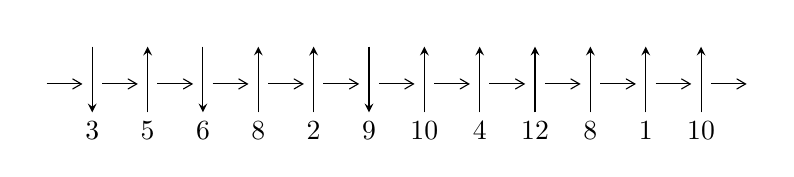
\begin{tikzpicture}[x=20pt, y=17pt]
	% nodes
	\node (C0) at (0, 0) {};
	\node (C1) at (1, 0) {};
	\node (C1U) at (1, +1) {};
	\node (C1D) at (1, -1) {3};

	\node (C2) at (2, 0) {};
	\node (C2U) at (2, +1) {};
	\node (C2D) at (2, -1) {5};

	\node (C3) at (3, 0) {};
	\node (C3U) at (3, +1) {};
	\node (C3D) at (3, -1) {6};

	\node (C4) at (4, 0) {};
	\node (C4U) at (4, +1) {};
	\node (C4D) at (4, -1) {8};

	\node (C5) at (5, 0) {};
	\node (C5U) at (5, +1) {};
	\node (C5D) at (5, -1) {2};

	\node (C6) at (6, 0) {};
	\node (C6U) at (6, +1) {};
	\node (C6D) at (6, -1) {9};

	\node (C7) at (7, 0) {};
	\node (C7U) at (7, +1) {};
	\node (C7D) at (7, -1) {10};

	\node (C8) at (8, 0) {};
	\node (C8U) at (8, +1) {};
	\node (C8D) at (8, -1) {4};

	\node (C9) at (9, 0) {};
	\node (C9U) at (9, +1) {};
	\node (C9D) at (9, -1) {12};

	\node (C10) at (10, 0) {};
	\node (C10U) at (10, +1) {};
	\node (C10D) at (10, -1) {8};

	\node (C11) at (11, 0) {};
	\node (C11U) at (11, +1) {};
	\node (C11D) at (11, -1) {1};

	\node (C12) at (12, 0) {};
	\node (C12U) at (12, +1) {};
	\node (C12D) at (12, -1) {10};
	\node (C13) at (13, 0) {};

	% arrows
	\draw[->,>={angle 60}]
	(C0) edge (C1) (C1) edge (C2) (C2) edge (C3) (C3) edge (C4) (C4) edge (C5) (C5) edge (C6) (C6) edge (C7) (C7) edge (C8) (C8) edge (C9) (C9) edge (C10) (C10) edge (C11) (C11) edge (C12) (C12) edge (C13) ;	\draw[->,>=stealth]
	(C1U) edge (C1D) (C2D) edge (C2U) (C3U) edge (C3D) (C4D) edge (C4U) (C5D) edge (C5U) (C6U) edge (C6D) (C7D) edge (C7U) (C8D) edge (C8U) (C9D) edge (C9U) (C10D) edge (C10U) (C11D) edge (C11U) (C12D) edge (C12U) ;
	\end{tikzpicture} \\
\hhline{~~} \\& 
\textbf{Solving Sequence} \\ \cline{2-2} 
 &
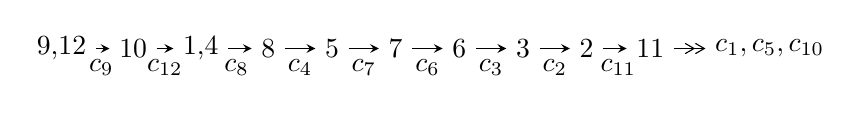
\begin{tikzpicture}[x=23pt, y=7pt]
	% node
	\node (A0) at (-1/8, 0) {9,12};
	\node (A1) at (1, 0) {10};
	\node (A2) at (33/16, 0) {1,4};
	\node (A3) at (25/8, 0) {8};
	\node (A4) at (33/8, 0) {5};
	\node (A5) at (41/8, 0) {7};
	\node (A6) at (49/8, 0) {6};
	\node (A7) at (57/8, 0) {3};
	\node (A8) at (65/8, 0) {2};
	\node (A9) at (73/8, 0) {11};
	\node (C1) at (1/2, -1) {$c_{9}$};
	\node (C2) at (3/2, -1) {$c_{12}$};
	\node (C3) at (21/8, -1) {$c_{8}$};
	\node (C4) at (29/8, -1) {$c_{4}$};
	\node (C5) at (37/8, -1) {$c_{7}$};
	\node (C6) at (45/8, -1) {$c_{6}$};
	\node (C7) at (53/8, -1) {$c_{3}$};
	\node (C8) at (61/8, -1) {$c_{2}$};
	\node (C9) at (69/8, -1) {$c_{11}$};
	\node (A10) at (11, 0) {$c_{1},c_{5},c_{10}$};

	% edge
	\draw[->,>=stealth]	
	(A0) edge (A1) (A1) edge (A2) (A2) edge (A3) (A3) edge (A4) (A4) edge (A5) (A5) edge (A6) (A6) edge (A7) (A7) edge (A8) (A8) edge (A9) ;
	\draw[->>,>={angle 60}]	
	(A9) edge (A10);
\end{tikzpicture} \\ 

\end{tabular} \\

\footnotetext{
The image of knot diagram is generated by the software ``\textbf{Draw programme}" developed by Andrew Bartholomew(\url{http://www.layer8.co.uk/maths/draw/index.htm\#Running-draw}), where we modified some parts for our purpose(\url{https://github.com/CATsTAILs/LinksPainter}).
}\phantom \\ \newline 
\centering \textbf{Ideals for irreducible components\footnotemark of $X_{\text{par}}$} 
 
\begin{align*}
I^u_{1}&=\langle 
2.36971\times10^{37} u^{58}-2.98861\times10^{38} u^{57}+\cdots+7.91576\times10^{35} b-5.88078\times10^{37},\\
\phantom{I^u_{1}}&\phantom{= \langle  }-2.37843\times10^{37} u^{58}+2.97918\times10^{38} u^{57}+\cdots+7.91576\times10^{35} a+4.16646\times10^{37},\\
\phantom{I^u_{1}}&\phantom{= \langle  }u^{59}-13 u^{58}+\cdots-10 u+1\rangle \\
I^u_{2}&=\langle 
a^2+b+a-1,\;a^4+a^3-2 a^2- a+2,\;u+1\rangle \\
I^u_{3}&=\langle 
b,\;- u^2 a+a^2+2 a u+3 u^2- a-5 u+4,\;u^3- u^2+1\rangle \\
I^u_{4}&=\langle 
a^5-3 a^4+4 a^2+b+a-1,\;a^6-3 a^5+5 a^3- a^2-2 a+1,\;u+1\rangle \\
\\
\end{align*}
\raggedright * 4 irreducible components of $\dim_{\mathbb{C}}=0$, with total 75 representations.\\
\footnotetext{All coefficients of polynomials are rational numbers. But the coefficients are sometimes approximated in decimal forms when there is not enough margin.}
\newpage
\renewcommand{\arraystretch}{1}
\centering \section*{I. $I^u_{1}= \langle 2.37\times10^{37} u^{58}-2.99\times10^{38} u^{57}+\cdots+7.92\times10^{35} b-5.88\times10^{37},\;-2.38\times10^{37} u^{58}+2.98\times10^{38} u^{57}+\cdots+7.92\times10^{35} a+4.17\times10^{37},\;u^{59}-13 u^{58}+\cdots-10 u+1 \rangle$}
\flushleft \textbf{(i) Arc colorings}\\
\begin{tabular}{m{7pt} m{180pt} m{7pt} m{180pt} }
\flushright $a_{9}=$&$\begin{pmatrix}1\\0\end{pmatrix}$ \\
\flushright $a_{12}=$&$\begin{pmatrix}0\\u\end{pmatrix}$ \\
\flushright $a_{10}=$&$\begin{pmatrix}1\\- u^2\end{pmatrix}$ \\
\flushright $a_{1}=$&$\begin{pmatrix}u\\- u^3+u\end{pmatrix}$ \\
\flushright $a_{4}=$&$\begin{pmatrix}30.0468 u^{58}-376.361 u^{57}+\cdots+458.241 u-52.6350\\-29.9366 u^{58}+377.552 u^{57}+\cdots-562.231 u+74.2920\end{pmatrix}$ \\
\flushright $a_{8}=$&$\begin{pmatrix}-97.4057 u^{58}+1230.14 u^{57}+\cdots-1933.17 u+261.759\\43.2007 u^{58}-546.214 u^{57}+\cdots+862.007 u-117.674\end{pmatrix}$ \\
\flushright $a_{5}=$&$\begin{pmatrix}81.4771 u^{58}-1025.89 u^{57}+\cdots+1495.08 u-200.409\\-51.6915 u^{58}+650.519 u^{57}+\cdots-976.689 u+133.016\end{pmatrix}$ \\
\flushright $a_{7}=$&$\begin{pmatrix}-125.970 u^{58}+1593.18 u^{57}+\cdots-2531.21 u+343.296\\44.4332 u^{58}-561.763 u^{57}+\cdots+916.403 u-125.970\end{pmatrix}$ \\
\flushright $a_{6}=$&$\begin{pmatrix}-81.5367 u^{58}+1031.41 u^{57}+\cdots-1614.81 u+217.326\\44.4332 u^{58}-561.763 u^{57}+\cdots+916.403 u-125.970\end{pmatrix}$ \\
\flushright $a_{3}=$&$\begin{pmatrix}48.4210 u^{58}-610.082 u^{57}+\cdots+892.310 u-120.705\\-39.1740 u^{58}+493.545 u^{57}+\cdots-742.666 u+101.904\end{pmatrix}$ \\
\flushright $a_{2}=$&$\begin{pmatrix}-39.3383 u^{58}+496.662 u^{57}+\cdots-738.577 u+96.1780\\0.368728 u^{58}-5.81774 u^{57}+\cdots+16.8281 u+0.227251\end{pmatrix}$ \\
\flushright $a_{11}=$&$\begin{pmatrix}- u^3\\u^5- u^3+u\end{pmatrix}$\\&\end{tabular}
\flushleft \textbf{(ii) Obstruction class $= -1$}\\~\\
\flushleft \textbf{(iii) Cusp Shapes $= -147.797 u^{58}+1865.74 u^{57}+\cdots-2967.33 u+417.985$}\\~\\
\newpage\renewcommand{\arraystretch}{1}
\flushleft \textbf{(iv) u-Polynomials at the component}\newline \\
\begin{tabular}{m{50pt}|m{274pt}}
Crossings & \hspace{64pt}u-Polynomials at each crossing \\
\hline $$\begin{aligned}c_{1}\end{aligned}$$&$\begin{aligned}
&u^{59}+31 u^{58}+\cdots+42 u-1
\end{aligned}$\\
\hline $$\begin{aligned}c_{2},c_{5}\end{aligned}$$&$\begin{aligned}
&u^{59}+5 u^{58}+\cdots+2 u-1
\end{aligned}$\\
\hline $$\begin{aligned}c_{3}\end{aligned}$$&$\begin{aligned}
&u^{59}-5 u^{58}+\cdots+4180 u-292
\end{aligned}$\\
\hline $$\begin{aligned}c_{4},c_{8}\end{aligned}$$&$\begin{aligned}
&u^{59}-2 u^{58}+\cdots+160 u-64
\end{aligned}$\\
\hline $$\begin{aligned}c_{6}\end{aligned}$$&$\begin{aligned}
&u^{59}-4 u^{58}+\cdots- u-1
\end{aligned}$\\
\hline $$\begin{aligned}c_{7},c_{10}\end{aligned}$$&$\begin{aligned}
&u^{59}+3 u^{58}+\cdots-1024 u-1024
\end{aligned}$\\
\hline $$\begin{aligned}c_{9},c_{12}\end{aligned}$$&$\begin{aligned}
&u^{59}+13 u^{58}+\cdots-10 u-1
\end{aligned}$\\
\hline $$\begin{aligned}c_{11}\end{aligned}$$&$\begin{aligned}
&u^{59}-13 u^{58}+\cdots+36 u-1
\end{aligned}$\\
\hline
\end{tabular}\\~\\
\newpage\renewcommand{\arraystretch}{1}
\flushleft \textbf{(v) Riley Polynomials at the component}\newline \\
\begin{tabular}{m{50pt}|m{274pt}}
Crossings & \hspace{64pt}Riley Polynomials at each crossing \\
\hline $$\begin{aligned}c_{1}\end{aligned}$$&$\begin{aligned}
&y^{59}- y^{58}+\cdots+2542 y-1
\end{aligned}$\\
\hline $$\begin{aligned}c_{2},c_{5}\end{aligned}$$&$\begin{aligned}
&y^{59}+31 y^{58}+\cdots+42 y-1
\end{aligned}$\\
\hline $$\begin{aligned}c_{3}\end{aligned}$$&$\begin{aligned}
&y^{59}-33 y^{58}+\cdots+4654184 y-85264
\end{aligned}$\\
\hline $$\begin{aligned}c_{4},c_{8}\end{aligned}$$&$\begin{aligned}
&y^{59}+40 y^{58}+\cdots-7168 y-4096
\end{aligned}$\\
\hline $$\begin{aligned}c_{6}\end{aligned}$$&$\begin{aligned}
&y^{59}-74 y^{58}+\cdots+5 y-1
\end{aligned}$\\
\hline $$\begin{aligned}c_{7},c_{10}\end{aligned}$$&$\begin{aligned}
&y^{59}+69 y^{58}+\cdots-21495808 y-1048576
\end{aligned}$\\
\hline $$\begin{aligned}c_{9},c_{12}\end{aligned}$$&$\begin{aligned}
&y^{59}-13 y^{58}+\cdots+36 y-1
\end{aligned}$\\
\hline $$\begin{aligned}c_{11}\end{aligned}$$&$\begin{aligned}
&y^{59}+79 y^{58}+\cdots+36 y-1
\end{aligned}$\\
\hline
\end{tabular}\\~\\
\newpage\flushleft \textbf{(vi) Complex Volumes and Cusp Shapes}
$$\begin{array}{c|c|c}  
\text{Solutions to }I^u_{1}& \I (\text{vol} + \sqrt{-1}CS) & \text{Cusp shape}\\
 \hline 
\begin{aligned}
u &= \phantom{-}0.784682 + 0.615628 I \\
a &= -0.577187 - 0.016841 I \\
b &= \phantom{-}0.241820 + 0.743409 I\end{aligned}
 & -3.71513 + 1.17573 I & \phantom{-0.000000 } 0 \\ \hline\begin{aligned}
u &= \phantom{-}0.784682 - 0.615628 I \\
a &= -0.577187 + 0.016841 I \\
b &= \phantom{-}0.241820 - 0.743409 I\end{aligned}
 & -3.71513 - 1.17573 I & \phantom{-0.000000 } 0 \\ \hline\begin{aligned}
u &= -0.989776 + 0.099585 I \\
a &= \phantom{-}3.21578 + 0.56260 I \\
b &= -0.477754 - 0.051833 I\end{aligned}
 & \phantom{-}1.37753 - 2.34293 I & \phantom{-0.000000 } 0 \\ \hline\begin{aligned}
u &= -0.989776 - 0.099585 I \\
a &= \phantom{-}3.21578 - 0.56260 I \\
b &= -0.477754 + 0.051833 I\end{aligned}
 & \phantom{-}1.37753 + 2.34293 I & \phantom{-0.000000 } 0 \\ \hline\begin{aligned}
u &= -0.510073 + 0.880995 I \\
a &= -0.25877 - 1.72077 I \\
b &= \phantom{-}0.43412 - 1.37809 I\end{aligned}
 & -5.44078 - 7.86618 I & \phantom{-0.000000 } 0 \\ \hline\begin{aligned}
u &= -0.510073 - 0.880995 I \\
a &= -0.25877 + 1.72077 I \\
b &= \phantom{-}0.43412 + 1.37809 I\end{aligned}
 & -5.44078 + 7.86618 I & \phantom{-0.000000 } 0 \\ \hline\begin{aligned}
u &= -0.270574 + 0.893509 I \\
a &= \phantom{-}0.10250 - 1.64711 I \\
b &= \phantom{-}0.067786 - 1.398240 I\end{aligned}
 & -6.44229 + 0.85012 I & \phantom{-0.000000 } 0 \\ \hline\begin{aligned}
u &= -0.270574 - 0.893509 I \\
a &= \phantom{-}0.10250 + 1.64711 I \\
b &= \phantom{-}0.067786 + 1.398240 I\end{aligned}
 & -6.44229 - 0.85012 I & \phantom{-0.000000 } 0 \\ \hline\begin{aligned}
u &= -0.425431 + 0.780931 I \\
a &= \phantom{-}0.11679 + 1.89599 I \\
b &= -0.291336 + 1.236710 I\end{aligned}
 & -2.39339 - 3.03762 I & \phantom{-}3.87633 + 3.56282 I \\ \hline\begin{aligned}
u &= -0.425431 - 0.780931 I \\
a &= \phantom{-}0.11679 - 1.89599 I \\
b &= -0.291336 - 1.236710 I\end{aligned}
 & -2.39339 + 3.03762 I & \phantom{-}3.87633 - 3.56282 I\\
 \hline 
 \end{array}$$\newpage$$\begin{array}{c|c|c}  
\text{Solutions to }I^u_{1}& \I (\text{vol} + \sqrt{-1}CS) & \text{Cusp shape}\\
 \hline 
\begin{aligned}
u &= -1.116770 + 0.010437 I \\
a &= -1.98632 + 0.23400 I \\
b &= \phantom{-}0.470430 + 0.432140 I\end{aligned}
 & \phantom{-}2.06662 + 1.38182 I & \phantom{-0.000000 } 0 \\ \hline\begin{aligned}
u &= -1.116770 - 0.010437 I \\
a &= -1.98632 - 0.23400 I \\
b &= \phantom{-}0.470430 - 0.432140 I\end{aligned}
 & \phantom{-}2.06662 - 1.38182 I & \phantom{-0.000000 } 0 \\ \hline\begin{aligned}
u &= \phantom{-}0.549864 + 0.598185 I \\
a &= -0.916575 + 0.380349 I \\
b &= \phantom{-}0.464850 + 0.860348 I\end{aligned}
 & -3.74978 + 1.11248 I & -1.95186 - 2.77586 I \\ \hline\begin{aligned}
u &= \phantom{-}0.549864 - 0.598185 I \\
a &= -0.916575 - 0.380349 I \\
b &= \phantom{-}0.464850 - 0.860348 I\end{aligned}
 & -3.74978 - 1.11248 I & -1.95186 + 2.77586 I \\ \hline\begin{aligned}
u &= \phantom{-}0.953228 + 0.719223 I \\
a &= \phantom{-}0.184839 + 0.296714 I \\
b &= \phantom{-}0.377691 - 0.510927 I\end{aligned}
 & -3.14792 + 4.18097 I & \phantom{-0.000000 } 0 \\ \hline\begin{aligned}
u &= \phantom{-}0.953228 - 0.719223 I \\
a &= \phantom{-}0.184839 - 0.296714 I \\
b &= \phantom{-}0.377691 + 0.510927 I\end{aligned}
 & -3.14792 - 4.18097 I & \phantom{-0.000000 } 0 \\ \hline\begin{aligned}
u &= -0.714347 + 0.335341 I \\
a &= -0.654918 - 0.346050 I \\
b &= -0.524386 - 0.448839 I\end{aligned}
 & \phantom{-}0.703685 + 0.029466 I & \phantom{-}6.19093 + 0.45904 I \\ \hline\begin{aligned}
u &= -0.714347 - 0.335341 I \\
a &= -0.654918 + 0.346050 I \\
b &= -0.524386 + 0.448839 I\end{aligned}
 & \phantom{-}0.703685 - 0.029466 I & \phantom{-}6.19093 - 0.45904 I \\ \hline\begin{aligned}
u &= -1.199090 + 0.275765 I \\
a &= -1.074520 - 0.161421 I \\
b &= \phantom{-}0.135658 - 1.049150 I\end{aligned}
 & \phantom{-}0.491598 - 1.220580 I & \phantom{-0.000000 } 0 \\ \hline\begin{aligned}
u &= -1.199090 - 0.275765 I \\
a &= -1.074520 + 0.161421 I \\
b &= \phantom{-}0.135658 + 1.049150 I\end{aligned}
 & \phantom{-}0.491598 + 1.220580 I & \phantom{-0.000000 } 0\\
 \hline 
 \end{array}$$\newpage$$\begin{array}{c|c|c}  
\text{Solutions to }I^u_{1}& \I (\text{vol} + \sqrt{-1}CS) & \text{Cusp shape}\\
 \hline 
\begin{aligned}
u &= \phantom{-}0.695422 + 0.239788 I \\
a &= -1.38241 - 0.41635 I \\
b &= \phantom{-}0.572360 + 1.047320 I\end{aligned}
 & -1.66131 + 8.15293 I & -0.65355 - 9.84045 I \\ \hline\begin{aligned}
u &= \phantom{-}0.695422 - 0.239788 I \\
a &= -1.38241 + 0.41635 I \\
b &= \phantom{-}0.572360 - 1.047320 I\end{aligned}
 & -1.66131 - 8.15293 I & -0.65355 + 9.84045 I \\ \hline\begin{aligned}
u &= -1.205170 + 0.432461 I \\
a &= \phantom{-}0.914841 + 0.101782 I \\
b &= \phantom{-}0.127563 + 1.275290 I\end{aligned}
 & -2.87819 + 2.67724 I & \phantom{-0.000000 } 0 \\ \hline\begin{aligned}
u &= -1.205170 - 0.432461 I \\
a &= \phantom{-}0.914841 - 0.101782 I \\
b &= \phantom{-}0.127563 - 1.275290 I\end{aligned}
 & -2.87819 - 2.67724 I & \phantom{-0.000000 } 0 \\ \hline\begin{aligned}
u &= -1.321580 + 0.290312 I \\
a &= \phantom{-}1.067150 + 0.011907 I \\
b &= -0.293061 + 1.285920 I\end{aligned}
 & -2.52983 - 5.56373 I & \phantom{-0.000000 } 0 \\ \hline\begin{aligned}
u &= -1.321580 - 0.290312 I \\
a &= \phantom{-}1.067150 - 0.011907 I \\
b &= -0.293061 - 1.285920 I\end{aligned}
 & -2.52983 + 5.56373 I & \phantom{-0.000000 } 0 \\ \hline\begin{aligned}
u &= \phantom{-}0.600679 + 0.233224 I \\
a &= \phantom{-}1.54602 + 0.26343 I \\
b &= -0.576951 - 0.942414 I\end{aligned}
 & \phantom{-}0.49550 + 3.30615 I & \phantom{-}3.00875 - 4.91162 I \\ \hline\begin{aligned}
u &= \phantom{-}0.600679 - 0.233224 I \\
a &= \phantom{-}1.54602 - 0.26343 I \\
b &= -0.576951 + 0.942414 I\end{aligned}
 & \phantom{-}0.49550 - 3.30615 I & \phantom{-}3.00875 + 4.91162 I \\ \hline\begin{aligned}
u &= \phantom{-}0.974533 + 0.944343 I \\
a &= -0.031805 + 0.507306 I \\
b &= \phantom{-}1.139410 - 0.115232 I\end{aligned}
 & -4.99278 + 3.48527 I & \phantom{-0.000000 } 0 \\ \hline\begin{aligned}
u &= \phantom{-}0.974533 - 0.944343 I \\
a &= -0.031805 - 0.507306 I \\
b &= \phantom{-}1.139410 + 0.115232 I\end{aligned}
 & -4.99278 - 3.48527 I & \phantom{-0.000000 } 0\\
 \hline 
 \end{array}$$\newpage$$\begin{array}{c|c|c}  
\text{Solutions to }I^u_{1}& \I (\text{vol} + \sqrt{-1}CS) & \text{Cusp shape}\\
 \hline 
\begin{aligned}
u &= \phantom{-}0.951583 + 0.976048 I \\
a &= \phantom{-}0.53629 - 1.61324 I \\
b &= -0.007849 - 1.197600 I\end{aligned}
 & -5.80099 + 0.66681 I & \phantom{-0.000000 } 0 \\ \hline\begin{aligned}
u &= \phantom{-}0.951583 - 0.976048 I \\
a &= \phantom{-}0.53629 + 1.61324 I \\
b &= -0.007849 + 1.197600 I\end{aligned}
 & -5.80099 - 0.66681 I & \phantom{-0.000000 } 0 \\ \hline\begin{aligned}
u &= -0.619938\phantom{ +0.000000I} \\
a &= -0.614103\phantom{ +0.000000I} \\
b &= -0.379392\phantom{ +0.000000I}\end{aligned}
 & \phantom{-}0.987384\phantom{ +0.000000I} & \phantom{-}10.0830\phantom{ +0.000000I} \\ \hline\begin{aligned}
u &= \phantom{-}1.008230 + 0.949033 I \\
a &= -0.79603 + 1.60808 I \\
b &= \phantom{-}0.203594 + 1.201400 I\end{aligned}
 & -5.61803 + 6.41573 I & \phantom{-0.000000 } 0 \\ \hline\begin{aligned}
u &= \phantom{-}1.008230 - 0.949033 I \\
a &= -0.79603 - 1.60808 I \\
b &= \phantom{-}0.203594 - 1.201400 I\end{aligned}
 & -5.61803 - 6.41573 I & \phantom{-0.000000 } 0 \\ \hline\begin{aligned}
u &= \phantom{-}0.938768 + 1.039960 I \\
a &= \phantom{-}0.071965 - 0.567951 I \\
b &= -1.352110 - 0.109099 I\end{aligned}
 & -8.53769 - 0.57441 I & \phantom{-0.000000 } 0 \\ \hline\begin{aligned}
u &= \phantom{-}0.938768 - 1.039960 I \\
a &= \phantom{-}0.071965 + 0.567951 I \\
b &= -1.352110 + 0.109099 I\end{aligned}
 & -8.53769 + 0.57441 I & \phantom{-0.000000 } 0 \\ \hline\begin{aligned}
u &= \phantom{-}0.830681 + 1.132630 I \\
a &= \phantom{-}0.214753 - 1.117890 I \\
b &= \phantom{-}0.48779 - 1.44380 I\end{aligned}
 & -9.96117 - 2.30085 I & \phantom{-0.000000 } 0 \\ \hline\begin{aligned}
u &= \phantom{-}0.830681 - 1.132630 I \\
a &= \phantom{-}0.214753 + 1.117890 I \\
b &= \phantom{-}0.48779 + 1.44380 I\end{aligned}
 & -9.96117 + 2.30085 I & \phantom{-0.000000 } 0 \\ \hline\begin{aligned}
u &= \phantom{-}0.79029 + 1.17849 I \\
a &= -0.187003 + 1.000660 I \\
b &= -0.63460 + 1.49501 I\end{aligned}
 & -13.0111 - 7.6806 I & \phantom{-0.000000 } 0\\
 \hline 
 \end{array}$$\newpage$$\begin{array}{c|c|c}  
\text{Solutions to }I^u_{1}& \I (\text{vol} + \sqrt{-1}CS) & \text{Cusp shape}\\
 \hline 
\begin{aligned}
u &= \phantom{-}0.79029 - 1.17849 I \\
a &= -0.187003 - 1.000660 I \\
b &= -0.63460 - 1.49501 I\end{aligned}
 & -13.0111 + 7.6806 I & \phantom{-0.000000 } 0 \\ \hline\begin{aligned}
u &= \phantom{-}1.05544 + 0.97189 I \\
a &= -0.008379 - 0.550553 I \\
b &= -1.335610 + 0.298327 I\end{aligned}
 & -8.15213 + 7.92720 I & \phantom{-0.000000 } 0 \\ \hline\begin{aligned}
u &= \phantom{-}1.05544 - 0.97189 I \\
a &= -0.008379 + 0.550553 I \\
b &= -1.335610 - 0.298327 I\end{aligned}
 & -8.15213 - 7.92720 I & \phantom{-0.000000 } 0 \\ \hline\begin{aligned}
u &= \phantom{-}0.91193 + 1.16122 I \\
a &= -0.388353 + 1.105940 I \\
b &= -0.33596 + 1.61613 I\end{aligned}
 & -14.8409 + 1.7634 I & \phantom{-0.000000 } 0 \\ \hline\begin{aligned}
u &= \phantom{-}0.91193 - 1.16122 I \\
a &= -0.388353 - 1.105940 I \\
b &= -0.33596 - 1.61613 I\end{aligned}
 & -14.8409 - 1.7634 I & \phantom{-0.000000 } 0 \\ \hline\begin{aligned}
u &= \phantom{-}1.14928 + 0.92975 I \\
a &= -1.11279 + 1.27285 I \\
b &= \phantom{-}0.61505 + 1.37396 I\end{aligned}
 & -8.89854 + 9.77362 I & \phantom{-0.000000 } 0 \\ \hline\begin{aligned}
u &= \phantom{-}1.14928 - 0.92975 I \\
a &= -1.11279 - 1.27285 I \\
b &= \phantom{-}0.61505 - 1.37396 I\end{aligned}
 & -8.89854 - 9.77362 I & \phantom{-0.000000 } 0 \\ \hline\begin{aligned}
u &= -0.217989 + 0.462422 I \\
a &= \phantom{-}0.352972 + 0.713663 I \\
b &= \phantom{-}0.883278 + 0.005614 I\end{aligned}
 & -1.01117 - 2.91966 I & \phantom{-}2.05527 + 5.38795 I \\ \hline\begin{aligned}
u &= -0.217989 - 0.462422 I \\
a &= \phantom{-}0.352972 - 0.713663 I \\
b &= \phantom{-}0.883278 - 0.005614 I\end{aligned}
 & -1.01117 + 2.91966 I & \phantom{-}2.05527 - 5.38795 I \\ \hline\begin{aligned}
u &= \phantom{-}1.18659 + 0.91747 I \\
a &= \phantom{-}1.16646 - 1.19440 I \\
b &= -0.73190 - 1.40356 I\end{aligned}
 & -11.6847 + 15.2392 I & \phantom{-0.000000 } 0\\
 \hline 
 \end{array}$$\newpage$$\begin{array}{c|c|c}  
\text{Solutions to }I^u_{1}& \I (\text{vol} + \sqrt{-1}CS) & \text{Cusp shape}\\
 \hline 
\begin{aligned}
u &= \phantom{-}1.18659 - 0.91747 I \\
a &= \phantom{-}1.16646 + 1.19440 I \\
b &= -0.73190 + 1.40356 I\end{aligned}
 & -11.6847 - 15.2392 I & \phantom{-0.000000 } 0 \\ \hline\begin{aligned}
u &= \phantom{-}1.14461 + 0.99662 I \\
a &= \phantom{-}0.96601 - 1.21203 I \\
b &= -0.49507 - 1.54081 I\end{aligned}
 & -14.0505 + 6.0390 I & \phantom{-0.000000 } 0 \\ \hline\begin{aligned}
u &= \phantom{-}1.14461 - 0.99662 I \\
a &= \phantom{-}0.96601 + 1.21203 I \\
b &= -0.49507 + 1.54081 I\end{aligned}
 & -14.0505 - 6.0390 I & \phantom{-0.000000 } 0 \\ \hline\begin{aligned}
u &= -0.442581 + 0.164163 I \\
a &= \phantom{-}0.19222 + 4.19542 I \\
b &= -0.094147 + 0.587865 I\end{aligned}
 & \phantom{-}0.76407 - 2.30945 I & -0.54330 + 7.28911 I \\ \hline\begin{aligned}
u &= -0.442581 - 0.164163 I \\
a &= \phantom{-}0.19222 - 4.19542 I \\
b &= -0.094147 - 0.587865 I\end{aligned}
 & \phantom{-}0.76407 + 2.30945 I & -0.54330 - 7.28911 I \\ \hline\begin{aligned}
u &= \phantom{-}0.321626 + 0.198610 I \\
a &= -1.71356 + 1.09600 I \\
b &= \phantom{-}0.744198 - 0.485695 I\end{aligned}
 & -0.01800 + 3.14526 I & \phantom{-}2.49375 - 2.79979 I \\ \hline\begin{aligned}
u &= \phantom{-}0.321626 - 0.198610 I \\
a &= -1.71356 - 1.09600 I \\
b &= \phantom{-}0.744198 + 0.485695 I\end{aligned}
 & -0.01800 - 3.14526 I & \phantom{-}2.49375 + 2.79979 I \\ \hline\begin{aligned}
u &= \phantom{-}0.375910 + 0.027813 I \\
a &= \phantom{-}2.24708 + 0.57233 I \\
b &= -0.625146 - 0.663345 I\end{aligned}
 & \phantom{-}1.37130 + 1.43610 I & \phantom{-}4.58545 - 3.40911 I \\ \hline\begin{aligned}
u &= \phantom{-}0.375910 - 0.027813 I \\
a &= \phantom{-}2.24708 - 0.57233 I \\
b &= -0.625146 + 0.663345 I\end{aligned}
 & \phantom{-}1.37130 - 1.43610 I & \phantom{-}4.58545 + 3.40911 I\\
 \hline 
 \end{array}$$\newpage\newpage\renewcommand{\arraystretch}{1}
\centering \section*{II. $I^u_{2}= \langle a^2+b+a-1,\;a^4+a^3-2 a^2- a+2,\;u+1 \rangle$}
\flushleft \textbf{(i) Arc colorings}\\
\begin{tabular}{m{7pt} m{180pt} m{7pt} m{180pt} }
\flushright $a_{9}=$&$\begin{pmatrix}1\\0\end{pmatrix}$ \\
\flushright $a_{12}=$&$\begin{pmatrix}0\\-1\end{pmatrix}$ \\
\flushright $a_{10}=$&$\begin{pmatrix}1\\-1\end{pmatrix}$ \\
\flushright $a_{1}=$&$\begin{pmatrix}-1\\0\end{pmatrix}$ \\
\flushright $a_{4}=$&$\begin{pmatrix}a\\- a^2- a+1\end{pmatrix}$ \\
\flushright $a_{8}=$&$\begin{pmatrix}- a^3- a^2+a+1\\a^3+a^2- a-1\end{pmatrix}$ \\
\flushright $a_{5}=$&$\begin{pmatrix}-1\\- a^2+2\end{pmatrix}$ \\
\flushright $a_{7}=$&$\begin{pmatrix}- a^3- a^2+a+1\\a^3+a^2- a-1\end{pmatrix}$ \\
\flushright $a_{6}=$&$\begin{pmatrix}0\\a^3+a^2- a-1\end{pmatrix}$ \\
\flushright $a_{3}=$&$\begin{pmatrix}a\\a^3+a^2- a-1\end{pmatrix}$ \\
\flushright $a_{2}=$&$\begin{pmatrix}- a^2+1\\a^3+2 a^2-1\end{pmatrix}$ \\
\flushright $a_{11}=$&$\begin{pmatrix}1\\-1\end{pmatrix}$\\&\end{tabular}
\flushleft \textbf{(ii) Obstruction class $= 1$}\\~\\
\flushleft \textbf{(iii) Cusp Shapes $= -3 a^3-2 a^2- a+10$}\\~\\
\newpage\renewcommand{\arraystretch}{1}
\flushleft \textbf{(iv) u-Polynomials at the component}\newline \\
\begin{tabular}{m{50pt}|m{274pt}}
Crossings & \hspace{64pt}u-Polynomials at each crossing \\
\hline $$\begin{aligned}c_{1},c_{6}\end{aligned}$$&$\begin{aligned}
&u^4-2 u^3+3 u^2- u+1
\end{aligned}$\\
\hline $$\begin{aligned}c_{2},c_{4}\end{aligned}$$&$\begin{aligned}
&u^4+u^2+u+1
\end{aligned}$\\
\hline $$\begin{aligned}c_{3}\end{aligned}$$&$\begin{aligned}
&u^4+3 u^3+4 u^2+3 u+2
\end{aligned}$\\
\hline $$\begin{aligned}c_{5},c_{8}\end{aligned}$$&$\begin{aligned}
&u^4+u^2- u+1
\end{aligned}$\\
\hline $$\begin{aligned}c_{7},c_{10}\end{aligned}$$&$\begin{aligned}
&u^4
\end{aligned}$\\
\hline $$\begin{aligned}c_{9},c_{11}\end{aligned}$$&$\begin{aligned}
&(u+1)^4
\end{aligned}$\\
\hline $$\begin{aligned}c_{12}\end{aligned}$$&$\begin{aligned}
&(u-1)^4
\end{aligned}$\\
\hline
\end{tabular}\\~\\
\newpage\renewcommand{\arraystretch}{1}
\flushleft \textbf{(v) Riley Polynomials at the component}\newline \\
\begin{tabular}{m{50pt}|m{274pt}}
Crossings & \hspace{64pt}Riley Polynomials at each crossing \\
\hline $$\begin{aligned}c_{1},c_{6}\end{aligned}$$&$\begin{aligned}
&y^4+2 y^3+7 y^2+5 y+1
\end{aligned}$\\
\hline $$\begin{aligned}c_{2},c_{4},c_{5}\\c_{8}\end{aligned}$$&$\begin{aligned}
&y^4+2 y^3+3 y^2+y+1
\end{aligned}$\\
\hline $$\begin{aligned}c_{3}\end{aligned}$$&$\begin{aligned}
&y^4- y^3+2 y^2+7 y+4
\end{aligned}$\\
\hline $$\begin{aligned}c_{7},c_{10}\end{aligned}$$&$\begin{aligned}
&y^4
\end{aligned}$\\
\hline $$\begin{aligned}c_{9},c_{11},c_{12}\end{aligned}$$&$\begin{aligned}
&(y-1)^4
\end{aligned}$\\
\hline
\end{tabular}\\~\\
\newpage\flushleft \textbf{(vi) Complex Volumes and Cusp Shapes}
$$\begin{array}{c|c|c}  
\text{Solutions to }I^u_{2}& \I (\text{vol} + \sqrt{-1}CS) & \text{Cusp shape}\\
 \hline 
\begin{aligned}
u &= -1.00000\phantom{ +0.000000I} \\
a &= \phantom{-}0.899232 + 0.400532 I \\
b &= -0.547424 - 1.120870 I\end{aligned}
 & -0.98010 + 7.64338 I & \phantom{-}6.92132 - 4.56334 I \\ \hline\begin{aligned}
u &= -1.00000\phantom{ +0.000000I} \\
a &= \phantom{-}0.899232 - 0.400532 I \\
b &= -0.547424 + 1.120870 I\end{aligned}
 & -0.98010 - 7.64338 I & \phantom{-}6.92132 + 4.56334 I \\ \hline\begin{aligned}
u &= -1.00000\phantom{ +0.000000I} \\
a &= -1.39923 + 0.32564 I \\
b &= \phantom{-}0.547424 + 0.585652 I\end{aligned}
 & \phantom{-}2.62503 + 1.39709 I & \phantom{-}14.5787 - 4.1375 I \\ \hline\begin{aligned}
u &= -1.00000\phantom{ +0.000000I} \\
a &= -1.39923 - 0.32564 I \\
b &= \phantom{-}0.547424 - 0.585652 I\end{aligned}
 & \phantom{-}2.62503 - 1.39709 I & \phantom{-}14.5787 + 4.1375 I\\
 \hline 
 \end{array}$$\newpage\newpage\renewcommand{\arraystretch}{1}
\centering \section*{III. $I^u_{3}= \langle b,\;- u^2 a+a^2+2 a u+3 u^2- a-5 u+4,\;u^3- u^2+1 \rangle$}
\flushleft \textbf{(i) Arc colorings}\\
\begin{tabular}{m{7pt} m{180pt} m{7pt} m{180pt} }
\flushright $a_{9}=$&$\begin{pmatrix}1\\0\end{pmatrix}$ \\
\flushright $a_{12}=$&$\begin{pmatrix}0\\u\end{pmatrix}$ \\
\flushright $a_{10}=$&$\begin{pmatrix}1\\- u^2\end{pmatrix}$ \\
\flushright $a_{1}=$&$\begin{pmatrix}u\\- u^2+u+1\end{pmatrix}$ \\
\flushright $a_{4}=$&$\begin{pmatrix}a\\0\end{pmatrix}$ \\
\flushright $a_{8}=$&$\begin{pmatrix}1\\0\end{pmatrix}$ \\
\flushright $a_{5}=$&$\begin{pmatrix}a\\0\end{pmatrix}$ \\
\flushright $a_{7}=$&$\begin{pmatrix}- u^2+1\\u^2- u-1\end{pmatrix}$ \\
\flushright $a_{6}=$&$\begin{pmatrix}- u\\u^2- u-1\end{pmatrix}$ \\
\flushright $a_{3}=$&$\begin{pmatrix}- a u\\2 u^2 a- a u-2 a\end{pmatrix}$ \\
\flushright $a_{2}=$&$\begin{pmatrix}- a u- u^2+2 u-1\\2 u^2 a- a u-2 a\end{pmatrix}$ \\
\flushright $a_{11}=$&$\begin{pmatrix}- u^2+1\\- u^2\end{pmatrix}$\\&\end{tabular}
\flushleft \textbf{(ii) Obstruction class $= 1$}\\~\\
\flushleft \textbf{(iii) Cusp Shapes $= 7 u^2 a-3 a u+3 u^2-8 a-9 u+10$}\\~\\
\newpage\renewcommand{\arraystretch}{1}
\flushleft \textbf{(iv) u-Polynomials at the component}\newline \\
\begin{tabular}{m{50pt}|m{274pt}}
Crossings & \hspace{64pt}u-Polynomials at each crossing \\
\hline $$\begin{aligned}c_{1},c_{3},c_{5}\end{aligned}$$&$\begin{aligned}
&(u^2- u+1)^3
\end{aligned}$\\
\hline $$\begin{aligned}c_{2}\end{aligned}$$&$\begin{aligned}
&(u^2+u+1)^3
\end{aligned}$\\
\hline $$\begin{aligned}c_{4},c_{8}\end{aligned}$$&$\begin{aligned}
&u^6
\end{aligned}$\\
\hline $$\begin{aligned}c_{6}\end{aligned}$$&$\begin{aligned}
&(u^3-3 u^2+2 u+1)^2
\end{aligned}$\\
\hline $$\begin{aligned}c_{7},c_{11}\end{aligned}$$&$\begin{aligned}
&(u^3+u^2+2 u+1)^2
\end{aligned}$\\
\hline $$\begin{aligned}c_{9}\end{aligned}$$&$\begin{aligned}
&(u^3- u^2+1)^2
\end{aligned}$\\
\hline $$\begin{aligned}c_{10}\end{aligned}$$&$\begin{aligned}
&(u^3- u^2+2 u-1)^2
\end{aligned}$\\
\hline $$\begin{aligned}c_{12}\end{aligned}$$&$\begin{aligned}
&(u^3+u^2-1)^2
\end{aligned}$\\
\hline
\end{tabular}\\~\\
\newpage\renewcommand{\arraystretch}{1}
\flushleft \textbf{(v) Riley Polynomials at the component}\newline \\
\begin{tabular}{m{50pt}|m{274pt}}
Crossings & \hspace{64pt}Riley Polynomials at each crossing \\
\hline $$\begin{aligned}c_{1},c_{2},c_{3}\\c_{5}\end{aligned}$$&$\begin{aligned}
&(y^2+y+1)^3
\end{aligned}$\\
\hline $$\begin{aligned}c_{4},c_{8}\end{aligned}$$&$\begin{aligned}
&y^6
\end{aligned}$\\
\hline $$\begin{aligned}c_{6}\end{aligned}$$&$\begin{aligned}
&(y^3-5 y^2+10 y-1)^2
\end{aligned}$\\
\hline $$\begin{aligned}c_{7},c_{10},c_{11}\end{aligned}$$&$\begin{aligned}
&(y^3+3 y^2+2 y-1)^2
\end{aligned}$\\
\hline $$\begin{aligned}c_{9},c_{12}\end{aligned}$$&$\begin{aligned}
&(y^3- y^2+2 y-1)^2
\end{aligned}$\\
\hline
\end{tabular}\\~\\
\newpage\flushleft \textbf{(vi) Complex Volumes and Cusp Shapes}
$$\begin{array}{c|c|c}  
\text{Solutions to }I^u_{3}& \I (\text{vol} + \sqrt{-1}CS) & \text{Cusp shape}\\
 \hline 
\begin{aligned}
u &= \phantom{-}0.877439 + 0.744862 I \\
a &= -0.111778 - 0.558770 I \\
b &= \phantom{-0.000000 } 0\end{aligned}
 & -3.02413 + 4.85801 I & \phantom{-}4.05323 - 9.17563 I \\ \hline\begin{aligned}
u &= \phantom{-}0.877439 + 0.744862 I \\
a &= -0.428020 + 0.376187 I \\
b &= \phantom{-0.000000 } 0\end{aligned}
 & -3.02413 + 0.79824 I & \phantom{-}7.63258 + 1.54443 I \\ \hline\begin{aligned}
u &= \phantom{-}0.877439 - 0.744862 I \\
a &= -0.111778 + 0.558770 I \\
b &= \phantom{-0.000000 } 0\end{aligned}
 & -3.02413 - 4.85801 I & \phantom{-}4.05323 + 9.17563 I \\ \hline\begin{aligned}
u &= \phantom{-}0.877439 - 0.744862 I \\
a &= -0.428020 - 0.376187 I \\
b &= \phantom{-0.000000 } 0\end{aligned}
 & -3.02413 - 0.79824 I & \phantom{-}7.63258 - 1.54443 I \\ \hline\begin{aligned}
u &= -0.754878\phantom{ +0.000000I} \\
a &= \phantom{-}1.53980 + 2.66701 I \\
b &= \phantom{-0.000000 } 0\end{aligned}
 & \phantom{-}1.11345 - 2.02988 I & \phantom{-}15.8142 - 4.6579 I \\ \hline\begin{aligned}
u &= -0.754878\phantom{ +0.000000I} \\
a &= \phantom{-}1.53980 - 2.66701 I \\
b &= \phantom{-0.000000 } 0\end{aligned}
 & \phantom{-}1.11345 + 2.02988 I & \phantom{-}15.8142 + 4.6579 I\\
 \hline 
 \end{array}$$\newpage\newpage\renewcommand{\arraystretch}{1}
\centering \section*{IV. $I^u_{4}= \langle a^5-3 a^4+4 a^2+b+a-1,\;a^6-3 a^5+5 a^3- a^2-2 a+1,\;u+1 \rangle$}
\flushleft \textbf{(i) Arc colorings}\\
\begin{tabular}{m{7pt} m{180pt} m{7pt} m{180pt} }
\flushright $a_{9}=$&$\begin{pmatrix}1\\0\end{pmatrix}$ \\
\flushright $a_{12}=$&$\begin{pmatrix}0\\-1\end{pmatrix}$ \\
\flushright $a_{10}=$&$\begin{pmatrix}1\\-1\end{pmatrix}$ \\
\flushright $a_{1}=$&$\begin{pmatrix}-1\\0\end{pmatrix}$ \\
\flushright $a_{4}=$&$\begin{pmatrix}a\\- a^5+3 a^4-4 a^2- a+1\end{pmatrix}$ \\
\flushright $a_{8}=$&$\begin{pmatrix}a^3-2 a^2- a+2\\- a^3+2 a^2+a-2\end{pmatrix}$ \\
\flushright $a_{5}=$&$\begin{pmatrix}- a^5+2 a^4+2 a^3-3 a^2-2 a+1\\a^4-2 a^3- a^2+2 a\end{pmatrix}$ \\
\flushright $a_{7}=$&$\begin{pmatrix}a^3-2 a^2- a+2\\- a^3+2 a^2+a-2\end{pmatrix}$ \\
\flushright $a_{6}=$&$\begin{pmatrix}0\\- a^3+2 a^2+a-2\end{pmatrix}$ \\
\flushright $a_{3}=$&$\begin{pmatrix}a\\a^3- a^2-2 a\end{pmatrix}$ \\
\flushright $a_{2}=$&$\begin{pmatrix}- a^4+a^3+2 a^2-1\\- a^5+3 a^4+a^3-5 a^2-2 a+1\end{pmatrix}$ \\
\flushright $a_{11}=$&$\begin{pmatrix}1\\-1\end{pmatrix}$\\&\end{tabular}
\flushleft \textbf{(ii) Obstruction class $= 1$}\\~\\
\flushleft \textbf{(iii) Cusp Shapes $= -5 a^4+8 a^3+8 a^2-8 a+4$}\\~\\
\newpage\renewcommand{\arraystretch}{1}
\flushleft \textbf{(iv) u-Polynomials at the component}\newline \\
\begin{tabular}{m{50pt}|m{274pt}}
Crossings & \hspace{64pt}u-Polynomials at each crossing \\
\hline $$\begin{aligned}c_{1},c_{6}\end{aligned}$$&$\begin{aligned}
&u^6-3 u^5+4 u^4-2 u^3+1
\end{aligned}$\\
\hline $$\begin{aligned}c_{2},c_{4}\end{aligned}$$&$\begin{aligned}
&u^6- u^5+2 u^4-2 u^3+2 u^2-2 u+1
\end{aligned}$\\
\hline $$\begin{aligned}c_{3}\end{aligned}$$&$\begin{aligned}
&(u^3- u^2+1)^2
\end{aligned}$\\
\hline $$\begin{aligned}c_{5},c_{8}\end{aligned}$$&$\begin{aligned}
&u^6+u^5+2 u^4+2 u^3+2 u^2+2 u+1
\end{aligned}$\\
\hline $$\begin{aligned}c_{7},c_{10}\end{aligned}$$&$\begin{aligned}
&u^6
\end{aligned}$\\
\hline $$\begin{aligned}c_{9},c_{11}\end{aligned}$$&$\begin{aligned}
&(u+1)^6
\end{aligned}$\\
\hline $$\begin{aligned}c_{12}\end{aligned}$$&$\begin{aligned}
&(u-1)^6
\end{aligned}$\\
\hline
\end{tabular}\\~\\
\newpage\renewcommand{\arraystretch}{1}
\flushleft \textbf{(v) Riley Polynomials at the component}\newline \\
\begin{tabular}{m{50pt}|m{274pt}}
Crossings & \hspace{64pt}Riley Polynomials at each crossing \\
\hline $$\begin{aligned}c_{1},c_{6}\end{aligned}$$&$\begin{aligned}
&y^6- y^5+4 y^4-2 y^3+8 y^2+1
\end{aligned}$\\
\hline $$\begin{aligned}c_{2},c_{4},c_{5}\\c_{8}\end{aligned}$$&$\begin{aligned}
&y^6+3 y^5+4 y^4+2 y^3+1
\end{aligned}$\\
\hline $$\begin{aligned}c_{3}\end{aligned}$$&$\begin{aligned}
&(y^3- y^2+2 y-1)^2
\end{aligned}$\\
\hline $$\begin{aligned}c_{7},c_{10}\end{aligned}$$&$\begin{aligned}
&y^6
\end{aligned}$\\
\hline $$\begin{aligned}c_{9},c_{11},c_{12}\end{aligned}$$&$\begin{aligned}
&(y-1)^6
\end{aligned}$\\
\hline
\end{tabular}\\~\\
\newpage\flushleft \textbf{(vi) Complex Volumes and Cusp Shapes}
$$\begin{array}{c|c|c}  
\text{Solutions to }I^u_{4}& \I (\text{vol} + \sqrt{-1}CS) & \text{Cusp shape}\\
 \hline 
\begin{aligned}
u &= -1.00000\phantom{ +0.000000I} \\
a &= -0.897438 + 0.201182 I \\
b &= \phantom{-}0.498832 - 1.001300 I\end{aligned}
 & \phantom{-}1.37919 - 2.82812 I & \phantom{-}10.11473 + 2.08748 I \\ \hline\begin{aligned}
u &= -1.00000\phantom{ +0.000000I} \\
a &= -0.897438 - 0.201182 I \\
b &= \phantom{-}0.498832 + 1.001300 I\end{aligned}
 & \phantom{-}1.37919 + 2.82812 I & \phantom{-}10.11473 - 2.08748 I \\ \hline\begin{aligned}
u &= -1.00000\phantom{ +0.000000I} \\
a &= \phantom{-}0.500000 + 0.273346 I \\
b &= -0.284920 - 1.115140 I\end{aligned}
 & -2.75839\phantom{ +0.000000I} & \phantom{-}1.72561 + 0.99756 I \\ \hline\begin{aligned}
u &= -1.00000\phantom{ +0.000000I} \\
a &= \phantom{-}0.500000 - 0.273346 I \\
b &= -0.284920 + 1.115140 I\end{aligned}
 & -2.75839\phantom{ +0.000000I} & \phantom{-}1.72561 - 0.99756 I \\ \hline\begin{aligned}
u &= -1.00000\phantom{ +0.000000I} \\
a &= \phantom{-}1.89744 + 0.20118 I \\
b &= -0.713912 + 0.305839 I\end{aligned}
 & \phantom{-}1.37919 + 2.82812 I & \phantom{-}9.65966 - 5.36114 I \\ \hline\begin{aligned}
u &= -1.00000\phantom{ +0.000000I} \\
a &= \phantom{-}1.89744 - 0.20118 I \\
b &= -0.713912 - 0.305839 I\end{aligned}
 & \phantom{-}1.37919 - 2.82812 I & \phantom{-}9.65966 + 5.36114 I\\
 \hline 
 \end{array}$$\newpage
\newpage\renewcommand{\arraystretch}{1}
\centering \section*{ V. u-Polynomials}
\begin{tabular}{m{50pt}|m{274pt}}
Crossings & \hspace{64pt}u-Polynomials at each crossing \\
\hline $$\begin{aligned}c_{1}\end{aligned}$$&$\begin{aligned}
&(u^2- u+1)^3(u^4-2 u^3+3 u^2- u+1)(u^6-3 u^5+4 u^4-2 u^3+1)\\
&\cdot(u^{59}+31 u^{58}+\cdots+42 u-1)
\end{aligned}$\\
\hline $$\begin{aligned}c_{2}\end{aligned}$$&$\begin{aligned}
&(u^2+u+1)^3(u^4+u^2+u+1)(u^6- u^5+2 u^4-2 u^3+2 u^2-2 u+1)\\
&\cdot(u^{59}+5 u^{58}+\cdots+2 u-1)
\end{aligned}$\\
\hline $$\begin{aligned}c_{3}\end{aligned}$$&$\begin{aligned}
&(u^2- u+1)^3(u^3- u^2+1)^2(u^4+3 u^3+4 u^2+3 u+2)\\
&\cdot(u^{59}-5 u^{58}+\cdots+4180 u-292)
\end{aligned}$\\
\hline $$\begin{aligned}c_{4}\end{aligned}$$&$\begin{aligned}
&u^6(u^4+u^2+u+1)(u^6- u^5+2 u^4-2 u^3+2 u^2-2 u+1)\\
&\cdot(u^{59}-2 u^{58}+\cdots+160 u-64)
\end{aligned}$\\
\hline $$\begin{aligned}c_{5}\end{aligned}$$&$\begin{aligned}
&(u^2- u+1)^3(u^4+u^2- u+1)(u^6+u^5+2 u^4+2 u^3+2 u^2+2 u+1)\\
&\cdot(u^{59}+5 u^{58}+\cdots+2 u-1)
\end{aligned}$\\
\hline $$\begin{aligned}c_{6}\end{aligned}$$&$\begin{aligned}
&((u^3-3 u^2+2 u+1)^2)(u^4-2 u^3+3 u^2- u+1)(u^6-3 u^5+\cdots-2 u^3+1)\\
&\cdot(u^{59}-4 u^{58}+\cdots- u-1)
\end{aligned}$\\
\hline $$\begin{aligned}c_{7}\end{aligned}$$&$\begin{aligned}
&u^{10}(u^3+u^2+2 u+1)^2(u^{59}+3 u^{58}+\cdots-1024 u-1024)
\end{aligned}$\\
\hline $$\begin{aligned}c_{8}\end{aligned}$$&$\begin{aligned}
&u^6(u^4+u^2- u+1)(u^6+u^5+2 u^4+2 u^3+2 u^2+2 u+1)\\
&\cdot(u^{59}-2 u^{58}+\cdots+160 u-64)
\end{aligned}$\\
\hline $$\begin{aligned}c_{9}\end{aligned}$$&$\begin{aligned}
&((u+1)^{10})(u^3- u^2+1)^2(u^{59}+13 u^{58}+\cdots-10 u-1)
\end{aligned}$\\
\hline $$\begin{aligned}c_{10}\end{aligned}$$&$\begin{aligned}
&u^{10}(u^3- u^2+2 u-1)^2(u^{59}+3 u^{58}+\cdots-1024 u-1024)
\end{aligned}$\\
\hline $$\begin{aligned}c_{11}\end{aligned}$$&$\begin{aligned}
&((u+1)^{10})(u^3+u^2+2 u+1)^2(u^{59}-13 u^{58}+\cdots+36 u-1)
\end{aligned}$\\
\hline $$\begin{aligned}c_{12}\end{aligned}$$&$\begin{aligned}
&((u-1)^{10})(u^3+u^2-1)^2(u^{59}+13 u^{58}+\cdots-10 u-1)
\end{aligned}$\\
\hline
\end{tabular}\newpage\renewcommand{\arraystretch}{1}
\centering \section*{ VI. Riley Polynomials}
\begin{tabular}{m{50pt}|m{274pt}}
Crossings & \hspace{64pt}Riley Polynomials at each crossing \\
\hline $$\begin{aligned}c_{1}\end{aligned}$$&$\begin{aligned}
&((y^2+y+1)^3)(y^4+2 y^3+\cdots+5 y+1)(y^6- y^5+\cdots+8 y^2+1)\\
&\cdot(y^{59}- y^{58}+\cdots+2542 y-1)
\end{aligned}$\\
\hline $$\begin{aligned}c_{2},c_{5}\end{aligned}$$&$\begin{aligned}
&(y^2+y+1)^3(y^4+2 y^3+3 y^2+y+1)(y^6+3 y^5+4 y^4+2 y^3+1)\\
&\cdot(y^{59}+31 y^{58}+\cdots+42 y-1)
\end{aligned}$\\
\hline $$\begin{aligned}c_{3}\end{aligned}$$&$\begin{aligned}
&(y^2+y+1)^3(y^3- y^2+2 y-1)^2(y^4- y^3+2 y^2+7 y+4)\\
&\cdot(y^{59}-33 y^{58}+\cdots+4654184 y-85264)
\end{aligned}$\\
\hline $$\begin{aligned}c_{4},c_{8}\end{aligned}$$&$\begin{aligned}
&y^6(y^4+2 y^3+3 y^2+y+1)(y^6+3 y^5+4 y^4+2 y^3+1)\\
&\cdot(y^{59}+40 y^{58}+\cdots-7168 y-4096)
\end{aligned}$\\
\hline $$\begin{aligned}c_{6}\end{aligned}$$&$\begin{aligned}
&(y^3-5 y^2+10 y-1)^2(y^4+2 y^3+7 y^2+5 y+1)\\
&\cdot(y^6- y^5+4 y^4-2 y^3+8 y^2+1)(y^{59}-74 y^{58}+\cdots+5 y-1)
\end{aligned}$\\
\hline $$\begin{aligned}c_{7},c_{10}\end{aligned}$$&$\begin{aligned}
&y^{10}(y^3+3 y^2+2 y-1)^2(y^{59}+69 y^{58}+\cdots-2.14958\times10^{7} y-1048576)
\end{aligned}$\\
\hline $$\begin{aligned}c_{9},c_{12}\end{aligned}$$&$\begin{aligned}
&((y-1)^{10})(y^3- y^2+2 y-1)^2(y^{59}-13 y^{58}+\cdots+36 y-1)
\end{aligned}$\\
\hline $$\begin{aligned}c_{11}\end{aligned}$$&$\begin{aligned}
&((y-1)^{10})(y^3+3 y^2+2 y-1)^2(y^{59}+79 y^{58}+\cdots+36 y-1)
\end{aligned}$\\
\hline
\end{tabular}
\vskip 2pc
\end{document}